\chapter{What Causes the Uncanny Valley?}   
\label{chap:4}
Soon after Masahiro Mori hypothesized the uncanny valley, the question of what causes the uncanny valley arose. Viewed simply, there can only be two answers to this question. Either the uncanny valley has an evolutionary origin and therefore develops at a very young age, or the uncanny valley arises through external influences over one's life experiences, therefore having a societal origin. 
\section{Explanatory Hypotheses of the Uncanny Valley}
According to Strait et al. \cite{childrens_responding}, there are two primary perceptually oriented hypotheses which thus support the evolutionary origin of the uncanny valley: the category ambiguity hypothesis and the feature atypicality hypothesis.\\
The category ambiguity hypothesis \cite{childrens_responding} is based on the difficulty, for us humans, in categorising very but not completely human-like entities. This categorisation has evolved in the course of our evolution and is one of the most basic human cognitive abilities. The valley-related discomfort is thus triggered when an entity cannot be categorised easily, which is the case at category boundaries, for example, the robot-human boundary. The category ambiguity hypothesis may also suggest that the uncanny valley is unavoidable due to the automatic categorisation humans experience when looking at different entities.\\
The feature atypicality hypothesis \cite{childrens_responding} argues that the uncanny valley originates in atypical features of figures that violate the expectations of their appearance or behaviour. An example of this would be a figure with a human-like head and a mechanical body. Such a figure would thus violate our expectations of how an actor should look or behave. Therefore this theory proposes that overall consistency regarding anthropomorphic or mechanomorphic features could avoid the uncanny valley effect.\\
The category ambiguity hypothesis and the feature atypicality hypothesis both explain the emergence of the uncanny valley through evolutionary processes. Otherwise, there is the theory that the uncanny valley arises through social influences over the course of a lifetime. Social triggers here could be, for example, the fear of humans being replaced by machines, which is spread by films or similar media. According to this theory, the uncanny valley would thus only develop with exposure to specific social influences and should therefore be less or not at all present in children or people who have been avoiding these social influences. 
\section{Differentiating Between the Explanatory Hypotheses}
In order to find the origin of the uncanny valley, we must first distinguish between the major opposing theories. Is the uncanny valley caused by our perception and has, therefore, an evolutionary origin or by social influences? After a consensus has been found in existing studies, it is possible to differentiate between either the two main hypotheses in the perceptually oriented direction, the category ambiguity hypothesis and the feature atypicality hypothesis, or between different influences that could cause the uncanny valley through social effects. The following discusses studies that have conducted experiments, testing whether the uncanny valley is already present in infants and children.
\subsection{Development of the Uncanny Valley in Infants}
A study by Lewkowicz et al. \cite{uncanny_infants} investigated the visual preferences of 6-, 8-, 10- and 12-month-old infants towards human faces, realistic avatar faces, and uncanny avatar faces to understand the synergy of evolutionary and developmental influences on the maturing of the uncanny valley effect. For their experiment, they chose 96 infants of mostly Caucasian phenotype and conducted three experiments in which they presented all possible pairs of three types of faces containing two human faces, two uncanny avatar faces and two realistic avatar faces, as seen in figure \ref{fig:uncannyInfants}, to the infants. 
\begin{wrapfigure}[13]{r}{0.6\textwidth} %this figure will be at the right
    \centering
    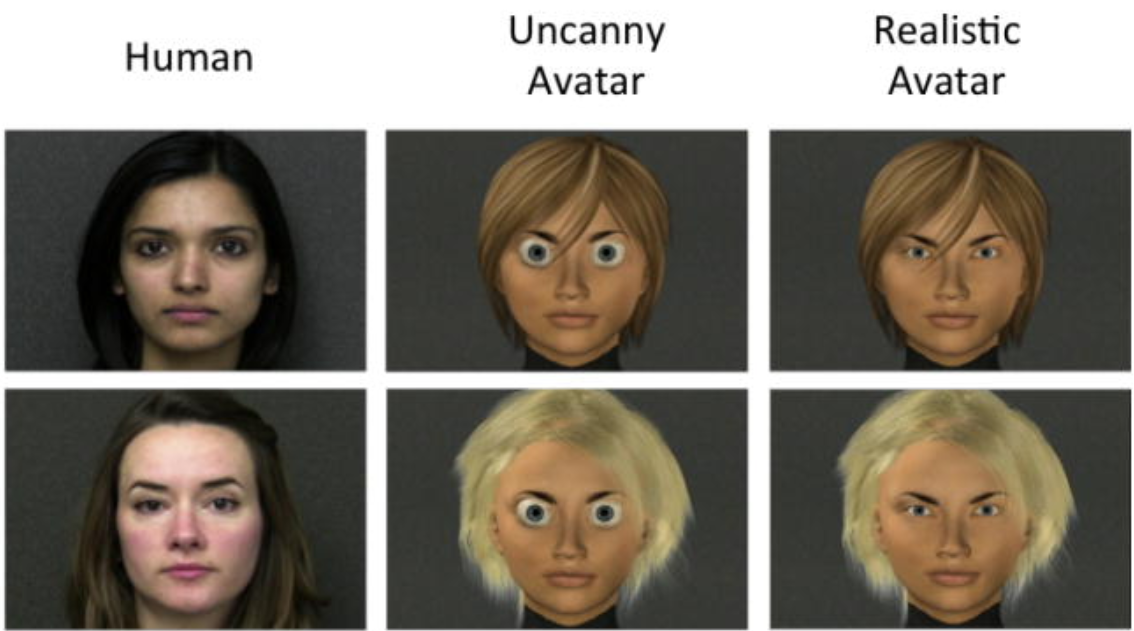
\includegraphics[width=0.6\textwidth]{graphics/uncanny_infants.png}
    \caption{Images of the three different types of faces.}
    \label{fig:uncannyInfants}
\end{wrapfigure}
In the first experiment, the uncanny avatar faces were combined with the human faces to monitor the infants' time to look at the different faces. The uncanny avatar faces were paired with the realistic avatar faces for the second experiment. The main difference between the realistic and uncanny faces were the unrealistically large eyes of the uncanny faces. Therefore, this experiment tested mainly whether infants are sensitive to large eyes by monitoring the time the infants looked at the different faces. In the third experiment, the realistic avatar faces were combined with the human faces to test if the response of the first experiment would be based on the eye size or if the infants were more sensitive to how closely the faces resembled a human prototype.\\
This study provides a fascinating new insight into the uncanny valley effect. The first experiment showed a dramatic shift in infant response to the uncanny avatar faces and human faces depending on their age. The 6-month-old infants preferred the uncanny avatar face instead of the human face, while the 12-month-old infants preferred the human face instead of the uncanny avatar face. Therefore, the uncanny valley effect is not yet present in the first six months of life, but it develops during the second half of the first year.\\
The second experiment confirmed that the infants are susceptible to eye size differences and that they preferred the faces with normal-sized eyes.\\
The results of the third experiment verified that the infants mainly paid attention to the eyes and did not recognise the synthetic nature of the realistic character. This further proved the study's main finding that infants looked less at the uncanny avatar because of the unusually large eyes.\\
In summary, this study suggests an interplay between the early influences on infant development and evolutionary mechanisms as the cause of the uncanny valley. Once infants have learned the prototype, they likely have sufficient perceptual experience to recognise irregularities in imperfect human-like entities, triggering the uncanny valley. It is also clear from previous studies that perceptual abilities are relatively crude at the start of life but improve rapidly during the first year \cite{Lewkowicz2009_perceptual_abilities,Pascalis2009_perceptual_abilities}. Specific developmental experiences of faces and emotions let their observers quickly learn to recognise abnormalities and aesthetic values of a face. As a result, faces that are abnormal/not human-like have a repulsive effect which causes an uncanny valley effect.\\\\
Matsuda et al. \cite{uncanny_infant_discrimination} conducted a similar study testing infants' discrimination against humanoid robots. In the study, an experiment showing three different types of agents to 42 infants aged between 6 to 14 months was conducted. The chosen visual stimuli consisted of three different black and white video clips, which pictured a human, an android and a mechanical robot performing a grasping action with their right hand, as shown in figure \ref{fig:uncannyInfantsDiscrimination}. The infants were each shown two different videos of the agents, which were played side by side. 
\newpage
The videos were paired into human and android, human and robot, and android and robot combinations. Each pair was shown to the infants four times for 10.5 seconds. During the experiment, the children were sitting on their parents' laps, who were instructed not to react either to the shown agents or to the infants. In order to analyse how the infants react to the different agents, their eye movements were monitored in real-time.
\begin{wrapfigure}{r}{0.6\textwidth} %this figure will be at the right
    \centering
    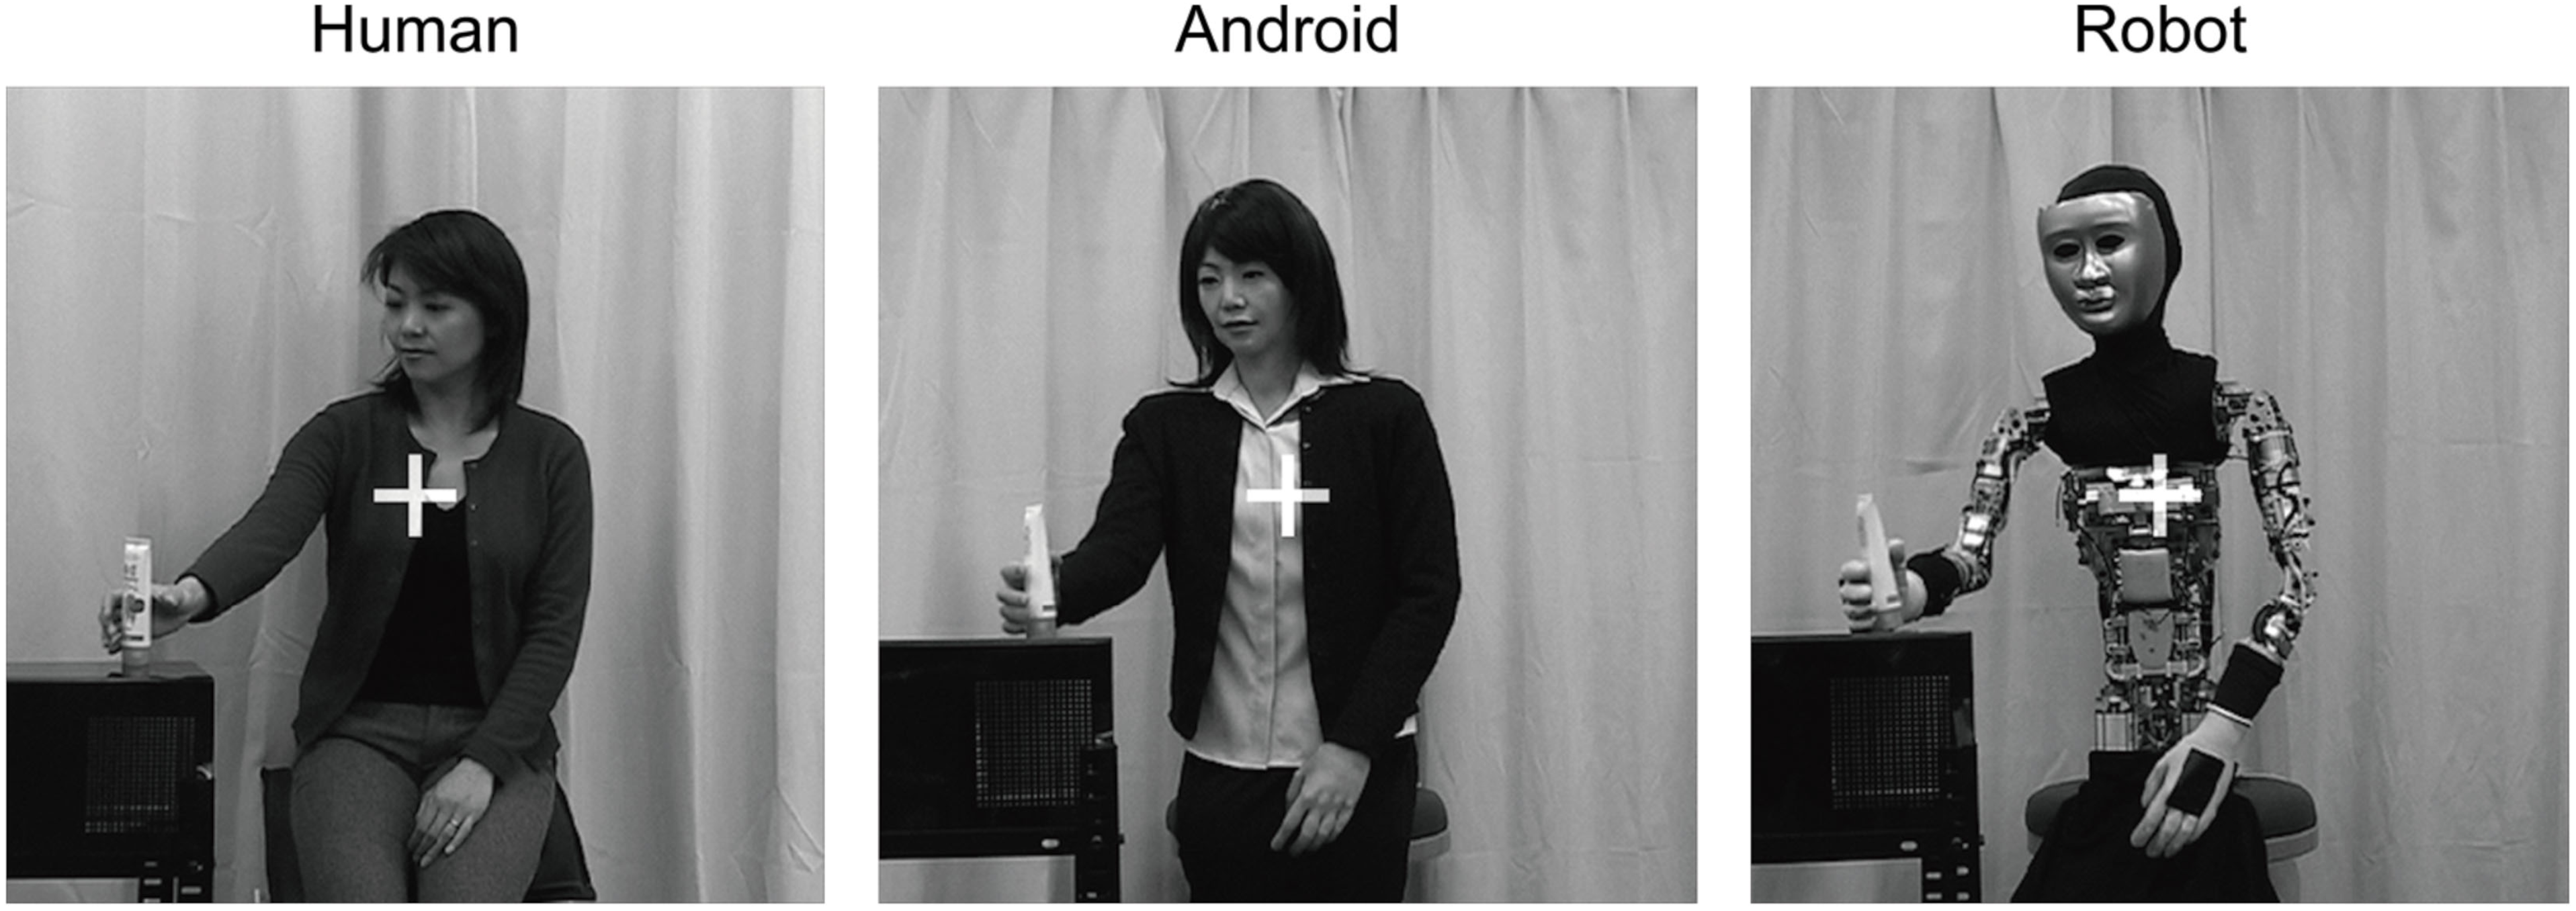
\includegraphics[width=0.6\textwidth]{graphics/uncanny_infants_discrimination.png}
    \caption{Images of the three different types of agents used.}
    \label{fig:uncannyInfantsDiscrimination}
\end{wrapfigure}
The experiment results show that the infants spent the longest time viewing the robot. In contrast to studies conducted with adults, there was no difference in the viewing time between the human and android agents. So this study suggests that infants up to 14 months of age do not yet have the perceptual abilities to distinguish between the human and android looking agents. However, it seems that they are already able to distinguish humans from robots. Since infants tend to observe novel objects, this could be a possible reason why they looked at the robots longer. In summary, this study did not find discrimination against androids in infants. From the study results, it can be suggested that the infants' perceptual abilities were not yet well enough to recognise the subtle differences between the human and android agents. As a result, the infants had not yet developed an uncanny valley effect.\\\\
When comparing the two studies, one can see certain similarities but also disagreements. The study by Lewkowicz et al. \cite{uncanny_infants} proposes that infants would learn the necessary perceptual abilities gradually in the second half of their first year of life to differentiate between human agents and human-like android agents. In contrast, the study by Matsuda et al. \cite{uncanny_infant_discrimination} could not find evidence that infants aged 14 months could differentiate sufficiently between the android agents and the human agents. However, they could already distinguish between humans and robots. By looking at the characters used by Lewkowicz et al. and Matsuda et al., one can see that the differences in the study by Matsuda et al. between the human and the uncanny agent are very subtle. On the contrary, the uncanny avatar from the study by Lewkowicz et al. can easily be distinguished from the human face. This may be the reason for the lack of response from the infants to the android agents in the study by Matsuda et al.. Concluding, it seems that the development of the uncanny valley goes hand in hand with the development of perceptual abilities in infants. This development seems to occur between the 6 and 14 months of an infant’s life, but the full development of these skills may depend on the individual’s developmental rate. This may explain the different results of the two studies. 
\newpage

\subsection{Observing the Uncanny Valley in Children}
To investigate the existence of the uncanny valley effect in children, Strait et al. \cite{childrens_responding} researched children's reactions, ranging from 5 to 10 years in age, to figures with different human-likeness and ordinary people. For the study, 80 children were recruited from a science museum. The children were shown a total of 24 different characters, which were divided into four categories of appearance: robot-like, humanoids with an atypic appearance, humanoids with an ambiguous appearance, and humans. The stimuli used for the experiment are depicted in figure \ref{fig:childrensRespondingAvatars}.
\begin{wrapfigure}{r}{0.5\textwidth} %this figure will be at the right
    \centering
    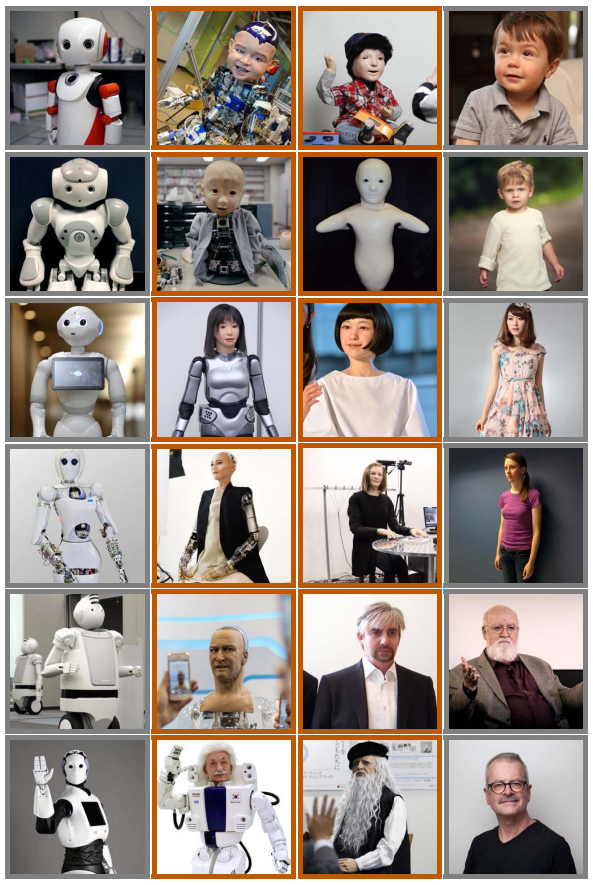
\includegraphics[width=0.5\textwidth]{graphics/childrens_responding_avatars.png}
    \caption{Images of the different figures used.}
    \label{fig:childrensRespondingAvatars}
\end{wrapfigure}
The six characters of the last column depict the humans; the remaining 18 are of little resemblance to humans, i.e. very robot-like to very human-like. To distinguish between the category ambiguity hypothesis and the feature atypicality hypothesis, the second column depicts humanoids with atypical features, such as a robot with a human head. The third column depicts humanoids with an ambiguous ontology.\\
The experiment consisted of two tasks.
First, the children had to complete an observation task in which they looked at the pictures for 12 seconds until the next picture appeared. During the 12 second observation time, the children could terminate at any time, which would take them to the following picture. This task was followed by a preference assessment in which the children were presented with four pictures from every category, mechanical, atypical, ambiguous  and human. The children were asked to indicate which of the four figures they liked most and which of the images they preferred the least.\\
The results of this study were analysed based on four indices, the dislike frequency and like frequency derived from the second task and the termination frequency and viewing duration from the first task.
The data from these indices showed that the children preferred the mechanical agents the most, followed by the real humans. 
However, they were averse to the very but not quite human-like entities, making their behaviour resemble the uncanny valley effect. Furthermore, from the dislike/like frequency data, a greater aversion towards the atypical characters than the ones with an ambiguous ontology could be identified. This study, therefore, showed that the aversion is driven more by atypicality than by ambiguity which thus supports the theory of the feature atypicality hypothesis. As there were no discernible differences in behaviour between the different age groups, the study assumed that the uncanny valley is of evolutionary origin and not triggered by social influences.\\

\section{External Influences on the Uncanny Valley}
From the discussed studies, it can be concluded that the uncanny valley has its origin in evolutionary mechanisms and evolves with the perceptual abilities in early childhood development. Based on research with children, Strait et al. \cite{childrens_responding} further inferred that there is a greater aversion towards atypical entities than entities with an ambiguous ontology, thus supporting the category ambiguity hypothesis. However, the study does not rule out the possibility that social influences may negatively or positively influence the uncanny valley. From the studies discussed, it can be concluded that an effect of social influences on the perception of the uncanny valley could have a significant role in the design and handling of social robots and similar human-like entities. For example, a positive influence would mean that the more people are exposed to the uncanny valley, the less they are influenced by it. However, the opposite effect, a strengthening of the uncanny valley through social influences, is also possible.\\
Alvarez Perez et al. \cite{prior_exposure_robots} investigated in their study if the uncanny valley also manifests with exposure to robots. For his study, two groups of participants were recruited, one with no previous exposure to robots and the other who had previously interacted with Nao, a humanoid robot from the French robot manufacturer Softbank Robotics. The procedure and stimuli were similar to the study by Strait et al.. The study concluded that the human-like actors triggered an uncanny valley in the participants. Furthermore, no attenuation of the uncanny valley could be shown with participants who had already been exposed to human-like robots. Both groups of participants experienced the uncanny valley effect in the same way. So this study could not find any improvement or worsening of the uncanny valley by previous exposure to robots. At this point, however, a need for future research can be identified. There is a lack of studies on the influence of external factors such as media, films or cultural and social differences on the uncanny valley.